\section{Задача}

Провести интеграционное тестирование программы, осуществляющей вычисление системы функций (в соответствии с вариантом).

\[
\begin{cases}
  (((((\sec(x) - \sec(x)) - \csc(x)) + \cos(x)) / (\sin(x) / \cot(x))) + (\cot(x) * \sin(x))), x \leq 0 \\
  (((((\log_5(x) * \log_2(x)) / \log_{10}(x)) * (\log_5(x) + \ln(x))) + (\log_3(x) - \log_{10}(x))) - (((\ln(x) * \ln(x)) - (\ln(x) * \log_5(x))) / \log_{10}(x))), x > 0
\end{cases}
\]

\section{Выполнение}

\begin{figure}[ht]
  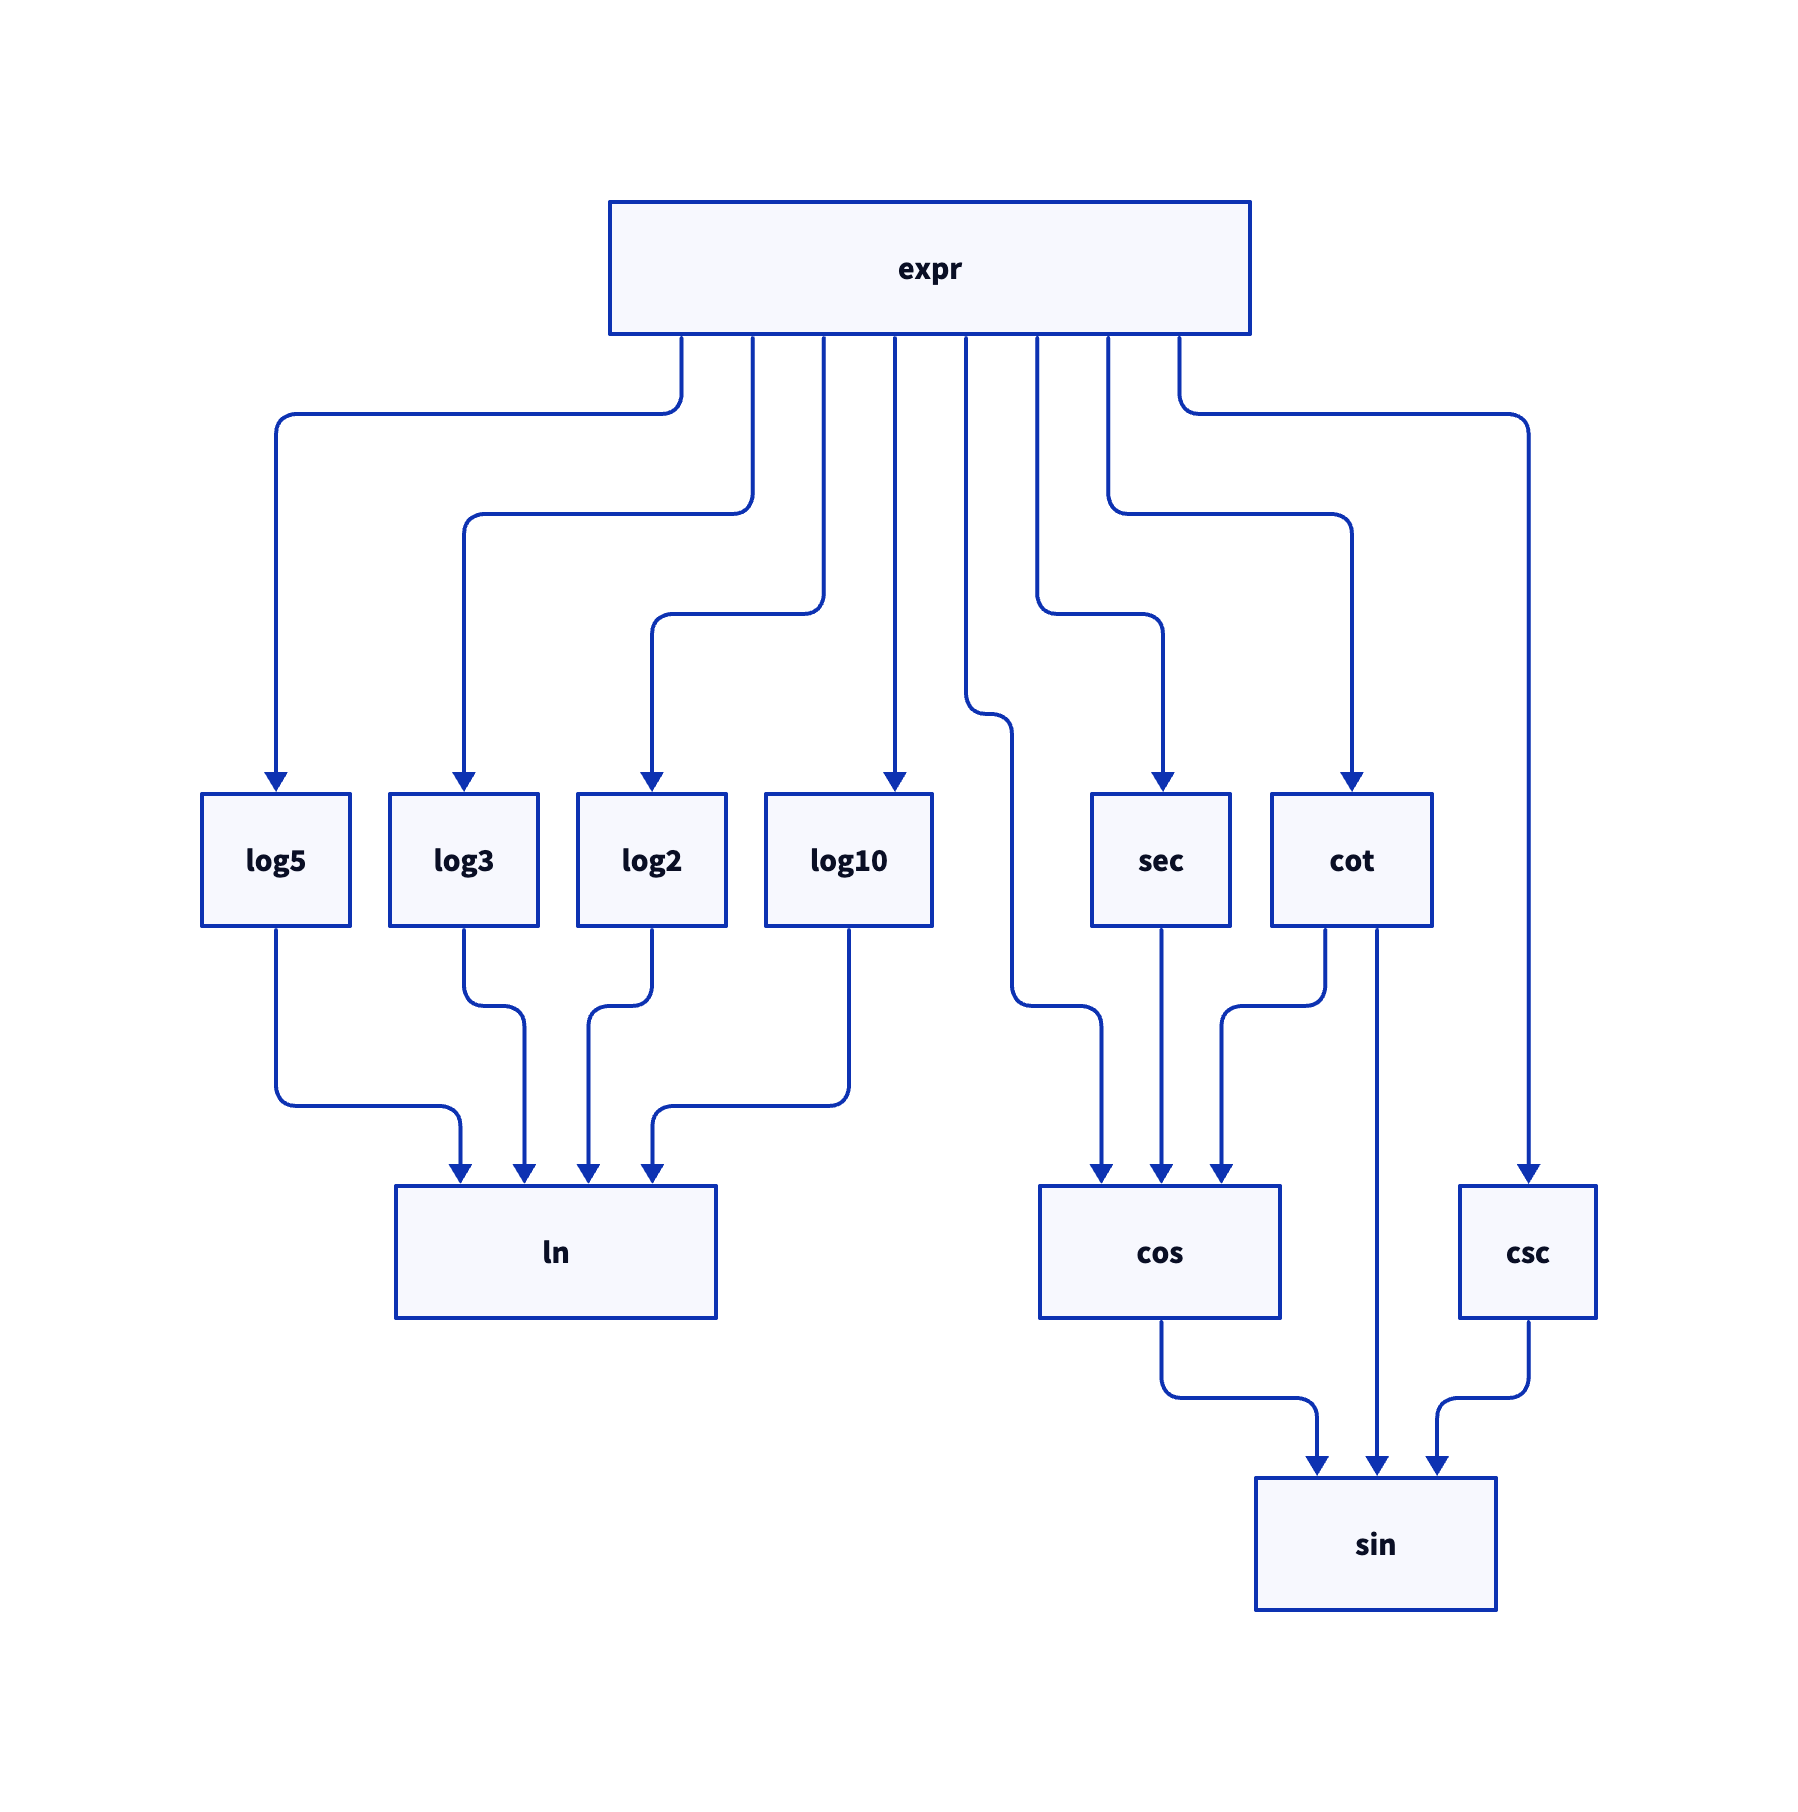
\includegraphics[width=\textwidth]{./assets/uml.png}
\end{figure}

\subsection{Описание тестового покрытия}

\subsubsection{Функция \(\sin\)}
\begin{itemize}
  \item Тестирование специальных углов \(0, \frac{\pi}{6}, \frac{\pi}{4}, \frac{\pi}{3}, \frac{\pi}{2}, \pi\)
  \item Проверка отрицательных входных значений
  \item Верификация свойства симметрии \(\sin(-x) = -\sin(x)\)
  \item Тестирование больших значений и периодичности
\end{itemize}

\subsubsection{Функция \(\ln\)}
\begin{itemize}
  \item Проверка специальных значений \(\ln(1) = 0, \ln(e) = 1\)
  \item Тестирование значений между 0 и 1
  \item Проверка значений больше 1
  \item Верификация свойства \(\ln(ab) = \ln(a) + \ln(b)\)
  \item Обработка недопустимых входных данных \(x \leq 0\)
\end{itemize}

\subsubsection{Функция \(\log\)}
\begin{itemize}
  \item Тестирование логарифмов с разными основаниями \(10, 2\) и другие
  \item Проверка свойства \(\log_b(b^n) = n\)
  \item Верификация связи с натуральным логарифмом \(\log_b(x) = \frac{\ln(x)}{\ln(b)}\)
  \item Обработка недопустимых входных данных
\end{itemize}

\subsubsection{Функция \(\cos\)}
\begin{itemize}
  \item Тестирование специальных углов
  \item Проверка свойства симметрии \(\cos(-x) = \cos(x)\)
  \item Верификация связи с \(\sin\): \(\cos(x) = \sin(x + \frac{\pi}{2})\)
\end{itemize}

\subsubsection{Функция \(\tan\)}
\begin{itemize}
  \item Тестирование специальных углов
  \item Проверка антисимметрии \(\tan(-x) = -\tan(x)\)
  \item Верификация связи с \(\sin\) и \(\cos\): \(\tan(x) = \frac{\sin(x)}{\cos(x)}\)
\end{itemize}

\subsubsection{Функция \(\sec\)}
\begin{itemize}
  \item Тестирование специальных углов
  \item Проверка симметрии \(\sec(-x) = \sec(x)\)
  \item Верификация связи с \(\cos\): \(\sec(x) = \frac{1}{\cos(x)}\)
\end{itemize}

\subsubsection{Функция \(\csc\)}
\begin{itemize}
  \item Тестирование специальных углов
  \item Проверка свойства \(\csc(-x) = -\csc(x)\)
  \item Верификация связи с \(\sin\): \(\csc(x) = \frac{1}{\sin(x)}\)
\end{itemize}

\subsubsection{Функция \texttt{complexExpression}}
\begin{itemize}
  \item Раздельное тестирование для \(x \leq 0\) и \(x > 0\)
  \item Проверка граничных значений
  \item Проверка взаимосвязей между функциями
\end{itemize}


Выбор тестового покрытия обоснован следующим:
\begin{itemize}
  \item Охват известных значений функций для проверки точности
  \item Проверка математических свойств для подтверждения корректности реализации
  \item Тестирование граничных случаев и исключительных ситуаций
  \item Проверка взаимосвязей между функциями, что также подтверждает корректность реализации
  \item Использование различных входных данных для обеспечения широкого покрытия функциональности
\end{itemize}

\begin{figure}
  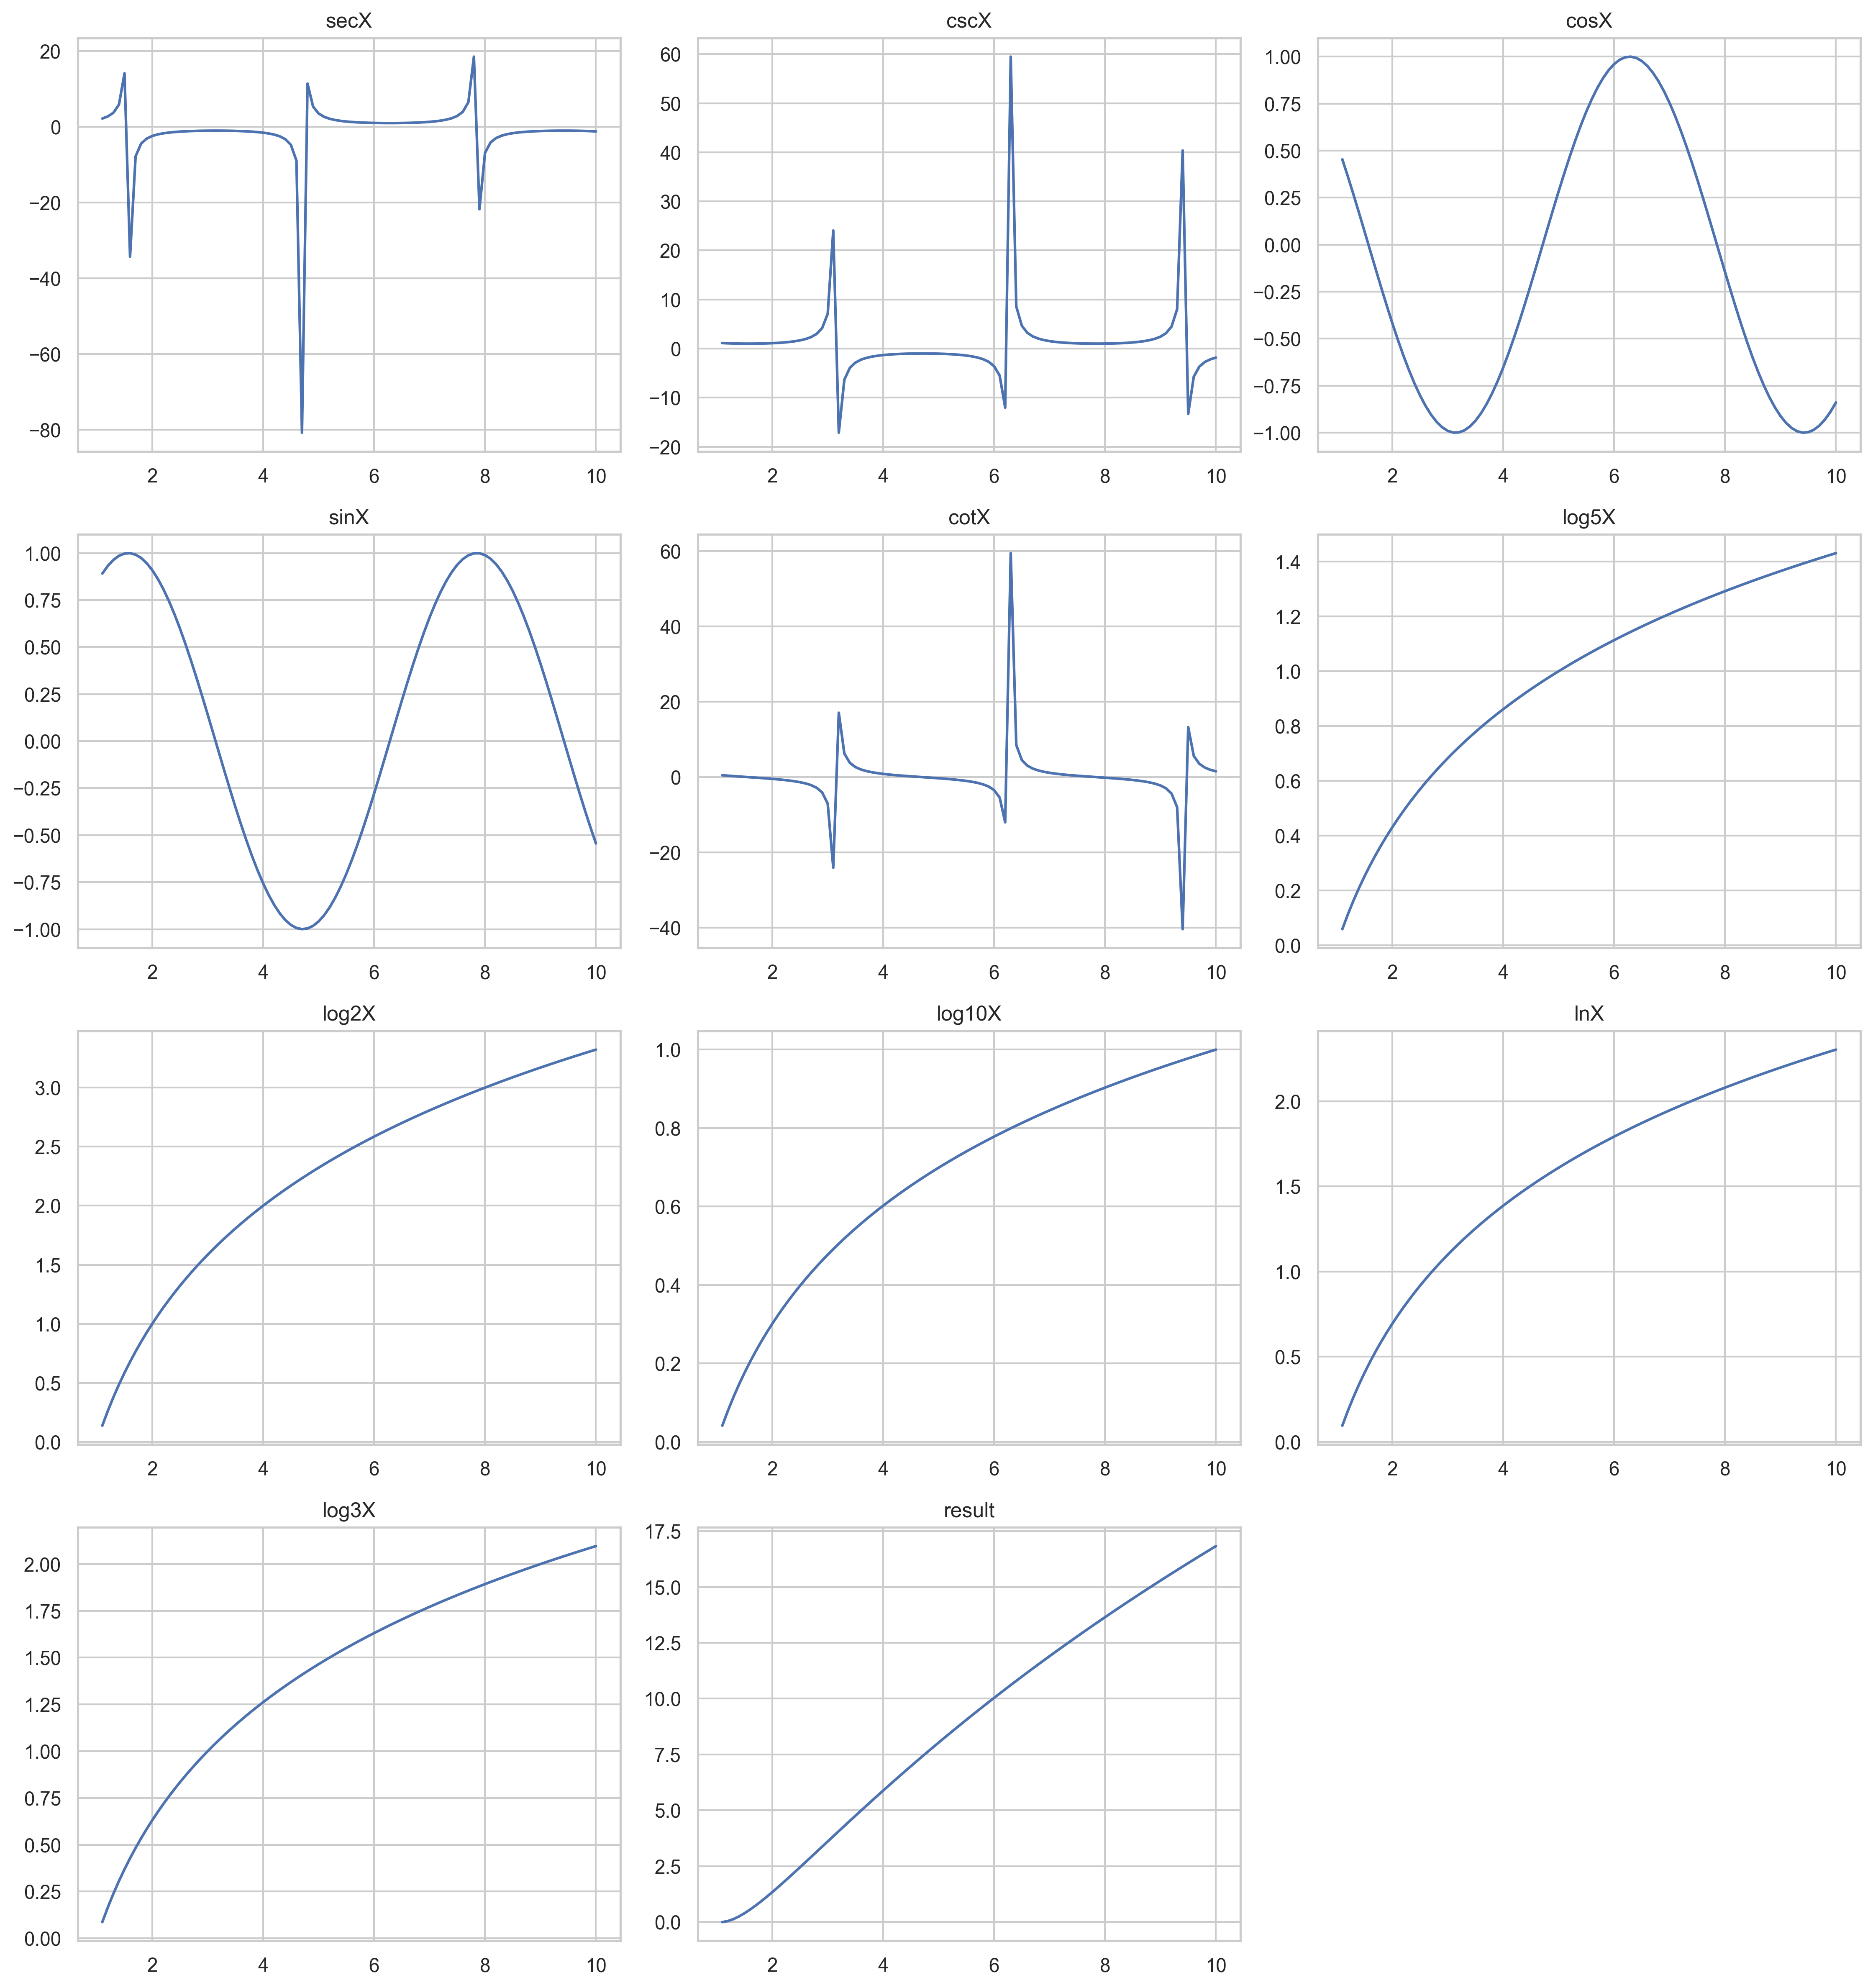
\includegraphics[width=\textwidth]{../plots/all_functions_subplots.png}
  \caption{График функций}
\end{figure}
